\chapter{Proposed Solution and Methodology}
\label{ch:methodology}

\section{Introduction}

\section{Proposed Solution}

The proposed solution for this project is inspired by the bus model that
supports the architecture of most commercial satellites. A standard software
and hardware platform provides common facilities required on all High-Altitude
flights – position tracking, internal data transfers and radio telemetry to the
ground station – allowing payloads (scientific instruments for example) to
only generate data and make it available to the platform.

\begin{figure}[H]
\includegraphics[width=0.35\textwidth]{payloadbus.pdf}
\centering
\caption{Platform architecture}
\end{figure}

The platform, or \textit{Payload Bus} is composed of the following components 
hardware and software components:

\begin{description}
    
\item[On Board Computer:] the computer that runs the flight software and
controls the data bus and all communications units (also called
\textit{Bus Controller}).

\item[Flight Software:] the firmware installed on the \textit{OBC}, that
controls the bus and the execution of the mission.

\item[Power Bus:] the hardware interface that provides electrical power to
payloads.

\item[Data Bus:] the hardware interface and software protocol through which
payloads communicate data to the flight computer.

\item[Navigation System:] the hardware (GNSS receiver) and software module used
by the flight software to keep track of the balloon's geographic coordinates and
altitude.

\item[Radio System:] the hardware (transmitter), protocols and software module
used by the \textit{OBC} to transmit collected data and metadata to the
ground station.

\item[Ground Segment:] the software required to record and decode the signal
received from the platform.
    
\end{description}

The following chapter describes the design processes used to develop and
integrate those components into a functioning prototype of the
\acrfull{ahabus}, and the methods used to test the viability and performance of
the design.

\section{Environment}

The proposed solution was designed to run on low-cost embedded platforms, and
the prototype was built around the Espressif ESP8266 micro-controller
(\acrlong{obc}). The radio link used a Radiometrix NTX2B transmitter
(\cite{radiometrix2012}), and an unnamed Software-Defined Radio receiver and
antenna.

The software packages used during the project were:

\begin{description}
    
\item[ESP OpenRTOS SDK] A FreeRTOS-based real-time kernel for the ESP8266.
\item[Clang/LLVM] C compiler for macOS (version 802.0.38).
\item[GQRX] macOS Software-Defined Radio application.
\item[dl-fldigi] digital radio decoding software.
\item[Textmate] Code editor.
\item[C (C99 standard)] Language used for all parts of \acrshort{ahabus}.
\item[Python 2.7] Language used for log file analysis

\end{description}

\section{Radio Communications}
\label{sec:radio-coms}

This section describes the design process that led to the radio communications
protocol used by the AHABus platform to send payload data and flight metadata
to the ground station. Its role is to ensure that arbitrary binary data – each
payload can use their own data format – as stably and reliably as possible. As
discussed in the following subsections, the design and implementation choice
were also driven by legal constraints: in the United Kingdom, airborne radio
transmitters are limited in frequency band (70cm wavelength) and power
(transmission power inferior to 10mW).

\subsection{Requirements}
\label{ssec:requirements}

Designing and building a communication protocol that can be relied up was an
important requirement for the rest of the project. Transmitting as much as
possible of a mission's scientific data is primordial in case the platform
is carried too far by winds and cannot be recovered after landing.

From the constraints discussed above, the requirements below were established
for the radio communications system:

\begin{itemize}
\item provide a system to transmit binary data.% DATA LINK
\item minimise the amount of overhead and bandwidth required.% ALL
\item allow multiple payload's data to be sent on the same link.% PACKET LAYER
\item provide stable transmissions on a low-power link.% FRAME LAYER
\item correct as many transmission-induced data errors as possible.% FRAME LAYER
\item allow ground crew to track the balloon's location over time.% PACKET LAYER
\end{itemize}

As stated in chapter \ref{ch:literature-review}, the United Kingdom's Office
of Communications restrict what frequencies can be used for airborne
radio transmissions, and how much power the transmissions can be sent at.
Those restrictions constrain what existing protocols can be used to transmit
arbitrary data over radio. This disqualifies existing packet radio protocols
that would have fulfilled most of the requirements, in use in other countries
like AX.25.
% TODO: mention Tx only, no Rx

Most UK-launched High Altitude Balloon missions make use of Radio-Teletype
(\textit{RTTY}) to send ASCII-encoded text. This was considered insufficient
for the purpose of a common platform for two main reasons: First, ASCII does
not handle binary data by default -- only some byte values would be displayed
as ASCII, while the rest would translate to non-printing characters. This leads
to data loss, unless the binary data is encoded in an ASCII-compatible format
like base64, which would require more bandwidth to send a similar amount of
data. Furthermore, ASCII alone does not provide either a way to multiplex data
coming from different payloads, or any kind of error checking or error
correction. This means that such facilities must be built on top of the
plain-text protocol.

RTTY itself functions in the same way as wired UART serial links. It can provide
some level of error checking if the transmission of a parity bit is enabled, but
it does not carry enough information to correct errors. Additionally, RTTY is
purely a link layer, and does not provide any kind of encapsulation necessary
for multiplexing data from different payloads.
%
% \subsection{Hardware Setup}
%
% The radio tra

\subsection{AHABus Radio Protocol}

The AHABus radio protocol was designed to match the requirements for the radio
system as closely as possible. While the specification presented in this section
is the last version, which was implemented in the AHABus prototype, some parts
of the protocol evolved or had to be changed during the prototyping process.
% TODO: Might not be necessary to say that here, given further sections

The protocol was designed in layers, some equivalent to the ones present in the
OSI model (\cite{Stallings1987}). This approach was chosen because it allows
some level of modularity – if a layer proves problematic, it can be swapped
for another with minimal impact on the other layers. Each layer fulfils a
specific purpose:

% TODO: Add some details about simplicity of the network topology

\begin{description}
\item[Link Layer:] The lowest-level layer's purpose is to establish a one-way
binary stream between the two end points of the radio link.

\item[Frame Layer:] The frame layer relies on the Link Layer to transmit its
data units, and provides reliability and error correction to higher-level 
layers.
% TODO: Add vocabulary maybe (ancillary)

\item[Packet Layer:] The packet layer is the highest-level layer. It provides
a way for multiple payloads' data to share bandwidth as well as metadata
transmission.
\end{description}

To avoid possible byte order conflicts between the architectures used on the
flight platform and the ground station, multi-byte values referred to in the
specification should always be transmitted as big-endian (most significant byte
first).

The design process and specification of each of those three layers is explained
in more details in the following sections.

\subsubsection{Link Layer}
\label{sssec:link-layer}

% TODO: add an introductory sentence?

While RTTY was not considered sufficient to cover fulfil the requirements of
the whole protocol, as shown in section \ref{ssec:requirements}, it fulfils the
simple requirements of the Link Layer: it can be used to send 8-bit bytes, one
by one, over a radio link.

RTTY functions like UART, over radio. Instead of using logical electrical levels
(5V for logical high, 0V for logical low), it uses Audio Frequency Shift Keying
(\textit{AFSK}): two audio tones separated by a frequency shift act as two
logical levels. When nothing is being transmitted, the line is held high. The
start of a byte is signalled by the \textit{start bit} (the line goes low),
followed by the eight \textit{data bits}, and one or two \textit{stop bits} (the
line is held high). After a byte has been sent, the line is held high again
until the next byte, or the next byte starts immediately.

Other existing protocols exist that can transmit data over radio audio signals,
like DominoEx or Olivia, sometimes with better transmission rates. RTTY was
preferred over them because the ESP8266 board used as OBC in the AHABus
prototype provides hardware support for UART, making it easier to implement and
reliable. Since the link layer is transparent to the frame and packet layers,
RTTY could be swapped for another protocol in the future with no impact on
those.

The valid encoding and decoding of a \acrshort{rtty} signal depends on the
chosen baud rate (the number of times the logical signal changes level). During
tests, the highest baud rate that allowed clear decoding of radio signals at
\SI{10}{mW} power rating was \SI{200}{bps}. Since each byte requires eleven
bits to be sent (one start bit, eight data bits and two stop bits), this
corresponds to a \(\frac{200}{11}=\SI{18.18}{Bps}\) bandwidth.

\subsubsection{Frame Layer}
\label{sssec:frame-layer}

The role of the frame layer is to provide higher-level layers with a reliable
data stream: the Link Layer discussed in section \ref{sssec:link-layer} will
send data bytes one after another, but it does not guarantee that the bytes are
received, or that noise on the channel (in this case, radio waves) have not
damaged the data between transmission and reception. Those are the two main
potential types of issues that the Frame Layer was designed to address.

Preventing complete data loss on a radio channel is only possible to a degree:
the signal-to-noise ratio is limited by multiple factors including transmission
power – limited in the United Kingdom – distance, other neighbouring
transmissions and line-of-sight. Those issues could have been mitigated in part
through solutions that were outside of this project's scope, like antennae
design. While this meant that some data loss could not be prevented, a solution
was required to detect occurrences of data loss, and identify which part of the
data was missing.

Identifying lost sections of an arbitrary stream of bytes without any form of
formatting is not possible: since it is not known in advance what data should
be expected, there is no model to which actual received data can be compared.
For this reason, the AHABus radio protocol was designed as a framed protocol:
the stream of data is divided in chunks of a set number of bytes, encapsulated
in \textit{frames} that contain the a sequence number used to track the position
of the chunk in the data stream.

The AHABus frame design was inspired by other frame-based protocols like the
CCSDS Space Packet/Frame protocol. Each frame is composed of two section: a
header, that contains metadata, and a payload containing the data carried by
that frame.

The only piece of metadata strictly required to be carried in a frame was its
sequence number. The frame format was designed to use a 16-bit integer to
represent the sequence number, as it allowed a large number of frames to be
sent in-between wrap-arounds of the number (when it becomes larger than 65,535).

To ensure that frames can be identified in the future, even if the format were
to evolve, the protocol version number was also added to the header format. At
the time of this writing, the protocol version was 0. If a future frame decoder
were to receive a frame indicating an old protocol version, it could be at
least signalled to the user, if not handled gracefully.

The resulting first version of the frame format is presented in figure
\ref{fig:frame-fmt-orig}.

\begin{figure}[H]
    \begin{center}
    \begin{bytefield}[bitwidth=0.5em]{64}
        \bitheader{0,8,24,40} \\
        \bitbox{8}{version} &
        \bitbox{16}{seq. number} &
        \bitbox{40}{data[253]}
    \end{bytefield}
    \end{center}
    \centering
    \caption{AHABus Frame Format – Version 1}
    \label{fig:frame-fmt-orig}
\end{figure}

This preliminary design proved impossible to work with: while it encapsulates
the required data and metadata, it does not provide any way to identify the
start or the end of a frame in a raw binary stream, which would have rendered
parsing an incoming frame stream impossible.

To solve this issue, a ``start sequence'' was added at the very beginning of
the frame. When parsing frames from a binary stream, the decoder must ignore
bytes until the start sequence (a single byte of value \texttt{0xAA} followed
by a single byte of value \texttt{0x5A}) occurs. Once the frame sequence is
detected, the frame's end is detected once 256 bytes have been received.

\begin{figure}[H]
    \begin{center}
    \begin{bytefield}[bitwidth=0.5em]{64}
        \bitheader{0,8,16,24,40} \\
        \bitbox{8}{\texttt{0xAA}} & \bitbox{8}{\texttt{0x5A}} & \bitbox{8}{version} &
        \bitbox{16}{seq. number} &
        \bitbox{24}{data[251]}
    \end{bytefield}
    \end{center}
    \centering
    \caption{AHABus Frame Format – Version 2}
    \label{fig:frame-fmt-2}
\end{figure}

The second version of the frame format shown in figure \ref{fig:frame-fmt-2}
fulfils one of its two design goals (detection of data loss). However, it does
not provide a way to detect and correct errors due to noise or interferences on
the radio channel.

The error-correction requirement led to the use of a Forward Error Correction
(\textit{FEC}) algorithm. FEC algorithms function by adding some amount of data
\(D\) to each message sent \(M\). In this case, the message includes both the
frame's header and its payload. \(D\) is computed by the encoder. The decoder
uses \(D\) to detect whether errors were introduced anywhere in the received
block \(M+D\), and correct those errors if their number is below the
algorithm's maximum.

% TODO: block diagram of the encoding-decoding chain

For the purpose of this project, Reed-Solomon(255,223) was chosen for multiple
reasons:

\begin{itemize}
    
\item The Reed-Solomon family of algorithms is widespread in its use, notably
in space communications systems – the Voyager probes used Reed-Solomon codes to
encode their images (\cite{Wicker1994}), the Space Data Links frames (devised
by \acrshort{esa} and \acrshort{ccsds}) use a variant of Reed-Solomon to
provide \acrshort{fec} (\cite{EuropeanCooperationforSpaceStandardization2010})
and the SSDV protocol, used in High-Altitude Balloon missions to transmit
low-resolution images, uses RS(255,223) with 256-byte frames (\cite{UKHAS2016}).

\item There were existing, well tested open-source implementation of that
specific variant of the Reed-Solomon encoders and decoders, which meant that
more time could be spent working on other parts of the project.

% TODO: Ask Ian, transparent might not be the right technical term

\item Reed-Solomon codes are transparent: the original data is not modified for
the purposes of error correction. This means that even if too many errors are
present for the \acrshort{fec} decoder to correct, the data can be manually
inspected and some of it can potentially be saved.
    
\end{itemize}

When applied to 8-bit \textit{symbols} (in this project's case, bytes),
Reed-Solomon codes can only handle blocks (Data and Error-Correction Codes) of
a length up to \(2^{8}-1 = 255\) bytes. The chosen variant, \(RS(223,255)\)
works on 223-byte messages, and adds 32 bytes of Error-Correction Codes at the
end to produce 255-byte blocks. This prompted slight changes in the frame
format: each frame being 256-byte long, one byte would not have been covered
by error correction.

The chosen solution was to not include the start sequence as part of the
error-corrected message. Since proper detection of that sequence is required
for the decoder to start parsing a frame, it would have been impossible to apply
\acrshort{fec} to a frame whose frame start sequence is corrupted.

\begin{figure}[H]
    \begin{center}
    \begin{bytefield}[bitwidth=1.8em]{20}
        \bitbox{1}{...} &
        \bitbox{8}{frame} &
        \bitbox{8}{frame} &
        \bitbox{3}{...}
    \end{bytefield}
    \end{center}
    \centering
    \caption{Frame stream with embedded start sequence}
    \label{fig:frame-sync-emb}
\end{figure}

The start sequence design had to be changed to occupy a single frame byte, as
opposed to two bytes in the second version of the frame format. Using a single
byte to detect the start of a frame was not deemed sufficient, since the
probably of that exact value occurring elsewhere in the binary stream would
have been fairly high. To mitigate this, the third and final version of the
frame format uses a single frame start marker (\texttt{0x5A}) at the beginning
of each frame, and each frame must be preceded by at least one synchronisation
byte (\texttt{0xAA}), inserted in the binary stream as shown in the lower half
of figure \ref{fig:frame-sync-extra}. The following 223 bytes in the frame
(starting with the protocol version number) are error-corrected, with the
frame's 32 trailing bytes.

\begin{figure}[H]
    \begin{center}
    \begin{bytefield}[bitwidth=1.8em]{20}
        \bitbox{1}{...} &
        \bitbox{1}{\texttt{AA}} &
        \bitbox{8}{frame} &
        \bitbox{1}{\texttt{AA}} &
        \bitbox{8}{frame} &
        \bitbox{1}{...}
    \end{bytefield}
    \end{center}
    \centering
    \caption{Frame stream with external synchronisation byte}
    \label{fig:frame-sync-extra}
\end{figure}

While this approach may seem wasteful since at least one extra byte must be
inserted in between each frame, it is to be noted that the same synchronisation
byte was previously part of each frame's 256 bytes, leading to a smaller amount
of data being encapsulated in each frame.

\begin{figure}[H]
    \begin{center}
    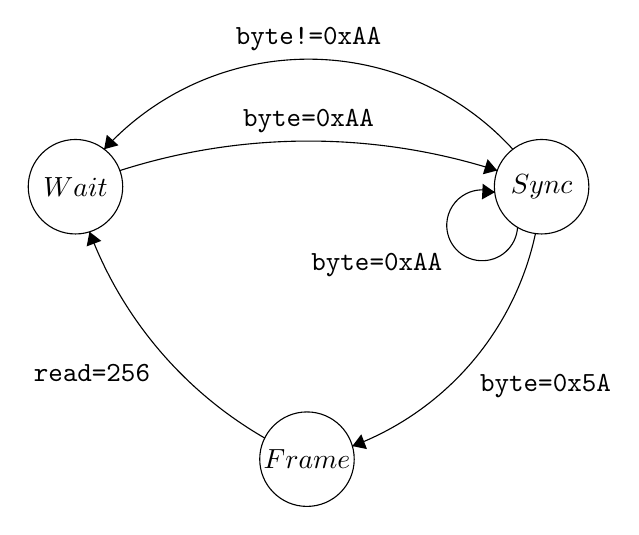
\begin{tikzpicture}[scale=0.2]
    \tikzstyle{every node}+=[inner sep=0pt]
    \draw [black] (23.9,-13.4) circle (3);
    \draw (23.9,-13.4) node {$Wait$};
    \draw [black] (53.5,-13.4) circle (3);
    \draw (53.5,-13.4) node {$Sync$};
    \draw [black] (38.6,-30.7) circle (3);
    \draw (38.6,-30.7) node {$Frame$};
    \draw [black] (26.719,-12.375) arc (107.79277:72.20723:39.209);
    \fill [black] (50.68,-12.37) -- (50.07,-11.65) -- (49.77,-12.61);
    \draw (38.7,-10) node [above] {$\texttt{byte=0xAA}$};
    \draw [black] (53.11,-16.371) arc (-12.09889:-69.37588:18.591);
    \fill [black] (41.48,-29.87) -- (42.41,-30.06) -- (42.05,-29.12);
    \draw (49.56,-26.05) node [right] {$\texttt{byte=0x5A}$};
    \draw [black] (35.918,-29.359) arc (-119.94439:-159.34576:25.489);
    \fill [black] (24.79,-16.26) -- (24.61,-17.19) -- (25.54,-16.84);
    \draw (28.67,-25.22) node [left] {$\texttt{read=256}$};
    \draw [black] (51.972,-15.968) arc (-3.02212:-291.02212:2.25);
    \draw (47.22,-18.39) node [left] {$\texttt{byte=0xAA}$};
    \fill [black] (50.53,-13.75) -- (49.76,-13.21) -- (49.71,-14.21);
    \draw [black] (25.724,-11.023) arc (137.60109:42.39891:17.571);
    \fill [black] (25.72,-11.02) -- (26.63,-10.77) -- (25.89,-10.1);
    \draw (38.7,-4.8) node [above] {$\texttt{byte!=0xAA}$};
    \end{tikzpicture}
    \end{center}
    \centering
    \caption{AHABus Frame Synchronisation State Machine}
    \label{fig:frame-fsm}
\end{figure}

Figure \ref{fig:frame-fsm} presents the finite state machine that
AHABus frame decoders must implement to detect frames in a binary
stream, and figure \ref{fig:frame-fmt-3} the final version of the
AHABus frame format.

% Go to the magic website http://madebyevan.com/fsm/

\begin{figure}[H]
    \begin{bytefield}{16}
        \bitheader{0,7,8,15} \\
        \begin{leftwordgroup}{Header}
            \bitbox{8}{\texttt{0x5A}} & \bitbox{8}{version} \\
            \bitbox{16}{sequence number}
        \end{leftwordgroup} \\
        \begin{leftwordgroup}{Payload}
            \wordbox{2}{data[]}
        \end{leftwordgroup} \\
        \begin{leftwordgroup}{FEC}
            \wordbox{2}{checksum[32]}
        \end{leftwordgroup}
    \end{bytefield}
    \centering
    \caption{AHABus Frame Format - Version 3}
    \label{fig:frame-fmt-3}
\end{figure}
 
%TODO: what's that worth? shouldn't it be at the end

Encapsulating the transmitted data adds overhead. If \(n\) is the size of a
chunk in bytes, and each frame adds \(m\) bytes of metadata, then only a
percentage \(\frac{n}{n+m}\) of the stream contains actual data. For reasons
explained further, the AHABus frames were chosen to be 256-byte
long. As shown previously, each frame also includes.

\subsubsection{Packet Layer}

The Packet Layer relies on the stable data stream provided by the Link and Frame
Layers, and was designed to allow the multiplexing of multiple payload's data as
well as the transmission of ancillary data required for the overall flight
management (platform's GNSS co-ordinates and altitude).

To achieve those goals, the AHABus protocol uses packets similar to frames. Each
packet encapsulates a chunk of data retrieved from a single payload. To that
end, packets were designed to be of variable length, to avoid unnecessary
padding, which would have wasted bandwidth. The data - referred to as the
packet's \textit{payload} – is preceded by the packet's header, which contains
information necessary to attribute the packet's data to a payload, indicate
the length of the packet, and carry the AHABus platform's location and altitude.

This design achieves multiplexing through time division: packets are chunked
and sent in frames one after the other, and can be dispatched to their
respective payload teams once decoded at the ground station. The main issue with
that method is that the protocol itself does not ensure that each payload gets
an even or fair share of the total bandwidth. As discussed in section
\ref{sec:flight-software}, this was solved in the flight software design.

\begin{figure}[H]
    \begin{bytefield}{32}
        \bitheader{0,7,8,15,16,23,24,31} \\
        \begin{leftwordgroup}{Header}
            \bitbox{8}{version} & \bitbox{8}{payload ID} &
            \bitbox{16}{length} \\
            \bitbox{32}{latitude} \\
            \bitbox{32}{longitude} \\
            \bitbox{16}{altitude} & \bitbox[lrt]{16}{}
        \end{leftwordgroup} \\
        \begin{leftwordgroup}{Payload}
            \wordbox[lrb]{3}{data[length]}
        \end{leftwordgroup}
    \end{bytefield}
    \centering
    \caption{AHABus Packet Format - Version 1}
    \label{fig:packet-fmt-1}
\end{figure}

Figure \ref{fig:packet-fmt-1} shows the first and current version of the AHABus
packet format. Like frame discussed in section \ref{sssec:frame-layer}, each
packet carries a version flag which was added to allow backwards compatibility,
were the protocol to evolve in the future.

The encoding of the metadata was chosen based on the physical constraints of
the information:

\begin{itemize}
\item Latitude and Longitudes can be both positive (North, East) or Negative
(South, West). At the equator, \SI{0.0001}{\degree} of longitude maps to
roughly eleven metres\footnotemark , and that distance decreases when moving
towards the poles, which was deemed precise enough for the project's purpose.
To avoid conflicts in floating-point mathematics conventions, and allow packet
encoders to be written for embedded platform without hardware floating point
support, latitude and longitude were designed to be multiplied by 10,000 and
transmitted as 32-bit precision signed integers.

\item Altitude is above zero for the whole mission duration, and cannot exceed
\SI{50000}{\meter}. Since a sub-metre precision is not required, and would
hardly be achievable with civilian GNSS receivers, it is encoded as a 16-bit
precision unsigned integer.

\end{itemize}

\footnotetext{
Earth circumference at the equator: \SI{40e6}{\meter}.
\(D_{\SI{0.0001}{\degree}} = 0.0001\times\frac{40\times{10^6}}{360}=\SI{11.1}{\meter}\)
}

The decision was made during the design process to align packet boundaries with
frame boundaries. This means that every time a new packet is sent through the
radio channel starts at the start of a new frame, instead of being inserted
in the middle of a frame, where the last packet stopped.

This approach leads to a loss in bandwidth: if a packet's length is not a 
multiple of the amount of data that a frame carry, the packet's last frame
will be padded with zeros instead of containing the start of the next packet.
However, it was deemed an acceptable tradeoff because of the issues that
non-aligned (contiguous) packets would present:

\begin{itemize}
\item If a packet's end does not match a frame's end, that frame cannot be
sent until the start of the next packet is known. This meant that the
transmission of most packet's last frames could be delayed for sometimes several
seconds until another packet is processed.

\item In the case where a frame is lost due to channel noise or interferences,
finding the start of the next packet would have been complicated, or required
a synchronisation mechanism similar to the one designed for AHABus frames.
Aligning packets instead makes such a system unnecessary, reducing the packet
header size and the complexity of packet decoders.
\end{itemize}

% TODO: Add diagram explaining aligment

\subsection{Initial Implementation and Testing}

To evaluate the protocol's viability, a full demonstration of an AHABus radio
stack was written. Its main goals were to provide a reference implementation of
a compliant encoder and decoder, validate the protocol's design process, and
test the algorithms used in a controlled environment before integrated testing.

The C language (ISO/IEC 9899:1999 standard) was chosen for the reference
implementation because of its widespread use, and its availability on most
micro-controller and embedded platforms, which would be used as AHABus flight
platforms. To render the code as portable and reusable as possible, care was
taken to limit the dependencies to a subset of the C language standard library,
and avoid use of dynamic memory allocation, which is often inefficient or
unavailable on embedded platforms.

To increase portability and ease of use further, the encoder and decoder read
and write data using user-supplied callback. This allows developers to import
the implementation files and use the library without editing, at the expense of
optimisation.
% TODO: Explain?

\subsubsection{Encoder}

Figure \ref{fig:encoder-flow} illustrate the data flow in the encoder.
In an attempt to use as little memory as possible, no intermediate
representation of the packet is created or stored. Instead, the header and
first chunk of the packet's data is written directly to a frame buffer. Once
the frame is fully constructed, its binary representation is written using the
user-provided callback. The buffer is then cleared, and the process is repeated
until all of the packet's payload has been framed. 

\begin{figure}[H]
\includegraphics[width=0.6\textwidth]{encoder-flow.pdf}
\centering
\caption{Encoder Data Flow}
\label{fig:encoder-flow}
\end{figure}

For testing purposes, a simple program was built that takes in user input,
uses the encoder to package that data and outputs the frame stream to the
UNIX standard output (\texttt{stdout}) so that the test decoder, discussed in
section \ref{sssec:rtx-decoder}, could parse it as input.

% TODO: more details? how much is required?
% TODO: add reference to appendix with code

\subsubsection{Decoder}
\label{sssec:rtx-decoder}

The decoding functions of the library were designed with threaded applications
in mind: the decoding function is given a callback called whenever a packet
is decoded, and never returns.

Decoding is done in a sequential way. Once the start of a frame has been
detected, the next 256 bytes are collected. Those 256 bytes are then checked
at increasing levels of details. Once a frame has been received, the first
action that the decoder runs is \acrlong{fec}. If all errors can be corrected,
the packet header is then extracted from the frame, as well as the beginning of
the packet's data. Subsequent frames are decoded the same way, except all of
their content is added to the packet's data, until the enough bytes have been
decoded to account for the packet's indicated length.

The user-provided callback function is invoked as soon as a full packet is
decoded. It is given a flag indicating whether any erroneous frames were
detected, so that potentially corrupted packets can be marked.

\section{Payload Bus}
\label{sec:payload-bus}

The Payload Bus is the hardware and software interface that is used by the
\acrfull{obc} to communicate with each payload carried on a mission.

\subsection{Requirements}

The requirements established for the payload bus were fairly simple: its only
role is to collect available data from each payload and make it available to
the flight software to process and transmit through the radio system.
Nonetheless a formal list of requirements was established:

\begin{itemize}
\item Provide a channel between payloads and the \acrshort{obc}.
\item Prevent multiple payloads from transmitting simultaneously.
\item Allow for different numbers of payloads with minimum changes.
\item Minimise the amount of Input/Output pins required on the \acrshort{obc}.
\end{itemize}

\subsection{Initial Prototypes}

Before a protocol was chosen, two different preliminary designs were devised
and experimented with outside of the full flight platform to ensure they were
viable, and which of the two was worth developing further.

\subsubsection{Serial Bus Interface}

The first experimental bus interface was designed around a Serial interface.
Serial interfaces (based on \acrshort{uart}) are only meant to connect two
devices, and require two data wires (one for each transmission direction). To
avoid requiring a pair of input/output pins on the \acrlong{obc} for each
connected payload, and simplify the electronic layout, all payloads were wired
in parallels on the same reception (Rx) and transmission (Rx) data lines. When
a payload had any data ready to be sent, it would transmit it using
\acrshort{uart} to the \acrshort{obc}, which would then store it in memory.

This configuration proved unusable. Because \acrshort{uart} is not designed
to handle multiple devices on the same connection endpoint, data would be
corrupted whenever two or more payloads were attempting to send data to the
\acrshort{obc}.

The chosen solution for this problem was to make four bus lines available to
each payload. In addition to the common Rx/Tx lines, each interface is composed
of a Communication Request Line ($\overline{CR}$) and a Communication Enable
Line ($\overline{CE}$). With this design, the communication sequence had to
be changed to the following:

\begin{enumerate}
\item When a payload is ready to send data, it pulls its $\overline{CR}$ line
low.
\item The \acrshort{obc} lists payloads that have raised CR. For each:
\begin{enumerate}
\item The \acrshort{obc} pulls the payload's $\overline{CE}$ line low.
\item The payload sends its data to the \acrshort{obc}.
\item The \acrshort{obc} releases the payload's $\overline{CE}$ line to high.
\item The payload releases its $\overline{CR}$ line to high.
\item The \acrshort{obc} processes the received data.
\end{enumerate}
\end{enumerate}

To ensure that non-cooperative payload could not attempt to send data when the
\acrshort{obc} had not addressed them through pulling the CE line high, a logic
AND gate (two NAND gates chained together as shown in figure \ref{fig:uart-nor})
was placed between the payload's Tx line and its $\overline{CE}$ line. With
this design, any signal on the Tx line could not get past the gate unless the
payload was being addressed, thus preventing a payload from corrupting
another's signal.

\begin{figure}[H]
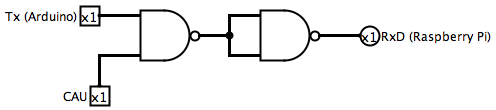
\includegraphics[width=0.6\textwidth]{serial-nand.png}
\centering
\caption{Payload Tx Line Protection}
\label{fig:uart-nor}
\end{figure}

This solution was tested using a Raspberry Pi 3 for the \acrlong{obc}, and an
Arduino UNO board for the payload. The system worked with the experimental
setup, and the \acrlong{obc} and the OBC were able to exchange data. However,
the design was deemed flawed because of the hardware requirements: while the Rx
and Tx lines are shared between all payloads, each still requires two I/O pins
on the \acrshort{obc} for the $\overline{CE}$ and $\overline{CR}$ lines. With
most micro-controllers exposing between 5 and 15 I/O pins, this would have
strongly limited how many payloads could have been connected at the same time.

\begin{figure}[H]
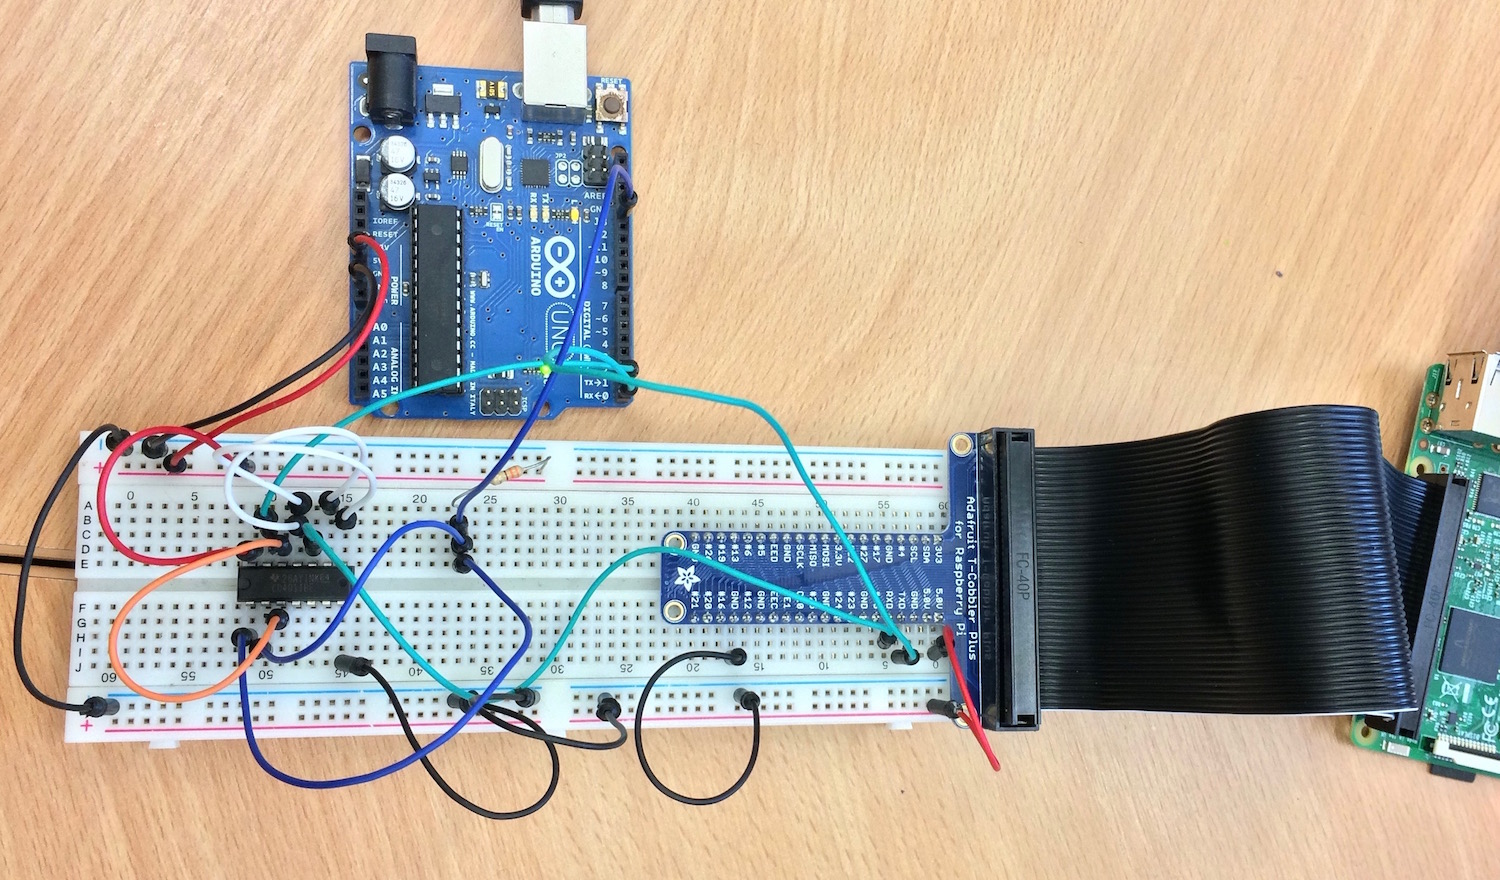
\includegraphics[width=0.6\textwidth]{serial-wires.jpg}
\centering
\caption{Payload Serial Bus Test Setup}
\label{fig:uart-nor}
\end{figure}

\subsubsection{\acrshort{i2c} Bus Interface}

% FIXME: move that to results?

The second experimental setup was much simpler: instead of using an hybrid
solution like the one described in the previous section, it relied on the
\acrshort{i2c} standard. The protocol was chosen because it provides a two-way
communication interface over two wires, for up to 127 devices. The major
difference with a \acrshort{uart} serial interface is that \acrshort{i2c} is
asymmetric: one device acts as the bus controller, and passive devices can
only receive or transmit data when addressed by it.

\subsection{AHABus Payload Bus Protocol}

After the two experiments described in in the previous sections, \acrshort{i2c}
was chosen as the payload bus's underlying protocol: it allows a large number of
payloads to be supported with only two lines (clock line, SCL, and data line,
SDA), and its controller/controllee paradigm allows the \acrshort{obc} to be
have complete control over which payload is allowed to transmit, and when.

The AHABus Payload Bus protocol was designed to work with a virtual register
system: each payload can be thought of like a memory array, and the bus
controller (the \acrshort{obc}) writes and reads data to and from addresses on
each payload. Addressing a specific payload on the bus, replying to the bus
controller and read/write operations are handled by the underlying
\acrshort{i2c} protocol (\cite{NXPSemiconductors2014}). Table
\ref{tab:bus-protocol-registers} gives the addresses, sizes and purposes of
each register. Multi-byte values are always encoded in big-endian order.

\begin{table}[h]
\begin{center}
\begin{tabular}{r||l l l}

address & size & name & description \\ \hline
\texttt{0x01} & 1 & Con. Flag & Set to \texttt{0xFF} by the \acrshort{obc} when  a connection is open. \\
\texttt{0x02} & 2 & Data Length & Number of data bytes available \\
\texttt{0x10} & - & data & Payload data exposed to the \acrshort{obc}

\end{tabular}
\end{center}
\caption {AHABus Payload Bus Protocol - Virtual Registers}
\label{tab:bus-protocol-registers}
\end{table}

When the bus controller starts polling a payload, a connection is opened by
writing \texttt{0xFF} to the Connection Flag register. To avoid data races,
payloads cannot change any of the registers values while the connection flag
is set. The controller then fetches two bytes from the Data Length register. If
there is no data to be collected (zero length), the controller closes the
connection by writing \texttt{0x00} in the connection flag.

If a non-zero amount of data is available, the controller can start requesting
it by sending \acrshort{i2c} read requests from address \texttt{0x10} onwards.
To be compatible with devices that only provide small transmissions buffers,
the controller cannot fetch more than 32 bytes at the same time. If there are
more than 32 bytes of data available, the controller will send multiple read
requests with increasing offsets from the base data address.

Once the data has been successfully collected, the controller closes the
connection by writing \texttt{0x00} in the connection flag.

\section{Flight Platform}
\label{sec:flight-software}

\subsection{Flight Software}

%TODO: formulation
The main role of the flight software is to link the subsystems discussed
previously and handle the data flowing through the system, from each payload's
raw data to the resulting radio frames. It is also responsible for keeping track
of the platform geographic co-ordinates and its altitude.

To avoid the added workload of designing and programming a real-time firmware
from nothing, the \acrfull{fcore}, \acrshort{ahabus}'s flight software, was
based upon FreeRTOS and the SDK provided by Espressif for the ESP8266
micro-controllers, which was used as the \acrshort{obc} for the prototype.

FreeRTOS is a real-time kernel that provides a prioritised task model: each task
is given a function (usually, an event loop) to run and a priority level. At
regular intervals, the kernel establishes a list of all the tasks that must run,
and gives processor time to the one with the highest priority. Such a
deterministic system is desirable for applications like \acrshort{ahabus}, which
must run on embedded devices with limited computing power, and where certain
actions must imperatively run at regular intervals. \acrshort{fcore} was
designed around three main tasks, along with the standalone radio subsystem.
Figure \ref{fig:fcore-arch} shows an overview of the the \acrshort{fcore}
architecture, and the component presented in the following sections.

\begin{figure}[H]
\includegraphics[width=0.6\textwidth]{fcore-arch.pdf}
\centering
\caption{\acrshort{fcore} architecture}
\label{fig:fcore-arch}
\end{figure}

\subsubsection{Payload Bus Task}

The payload bus subsystem was designed so that each payload connected to the
platform is given a unique identifier, which is also its address on the
\acrshort{i2c} bus. To avoid errors emanating from one payload to propagate
and take the whole payload bus offline, each payload is assigned a Payload
Bus Task.

A Bus Tasks runs at a fixed interval, configured at compile time depending on
the payload's priority level, as discussed in more details in section
\ref{sssec:conf-file}. The task establishes a connection with the payload using
the \acrshort{ahabus} payload bus protocol. If data is available, it is
collected into a temporary buffer and a packet with the platform's cached
geographical coordinates is created and sent to the radio submodule.

While the ESP8266 micro-controller does not have any hardware \acrshort{i2c}
support, the FreeRTOS SDK provides an implementation based on hardware timers
that was used for bus operations. As discussed in the results (section
\ref{ssec:results-bus}), the library had to be modified to extend the
\acrshort{i2c} clock stretch timeout to \SI{100000}{\micro\second}, so that
payloads with relatively slow processors had enough time to reply to commands.

Because all the payload bus tasks run at the same priority level, there was a
possibility that a payload's task could take control of the kernel while another
was still communicating with its own payload. To avoid this, the portion of the
code that handles communications over the bus and packetisation was marked
as critical, preventing FreeRTOS from triggering a context switch until all data
is collected.

\subsubsection{System Health Task}

The system task runs at fixed intervals to check the status of each subsystem
and create a system health message, sent to the ground station through the
radio subsystem. It was assigned the highest priority level, so that even if a
subsystem were to fail and not explicitly release control, FreeRTOS would give
the System Task the execution context, thus allowing health packets to be sent
to the ground station.

The health of each subsystem is stored globally, and each system can indicate
an issue by modifying its entry. There are four health states that subsystems
can have, represented each by a single ASCII character: booting (B), up (U),
recovering (R) and down (D). Each system is flagged as booting on startup.
Payloads are flagged as recovering if the payload attempted to transmit more
data than it is allowed, and down if it failed to respond to polling. the
\acrshort{gnss} subsystem is flagged as recovering if no valid position fix was
received from the receiver, and down if the received messages were not parsed
correctly.

Health messages were designed to be human-readable: this improves the chances
that ground teams can understand the status of the platform, even if the
message's packet and frame were to be corrupted beyond the Frame Layer's
\acrshort{fec} limits.

The message is sent as a list of comma-separated entries. Each entry starts
with a letter indicating its type (G for the \acrshort{gnss} subsystem, P for
payloads). In the case of payloads, the type is followed by the payload's
identifier as a two-character hexadecimal number. The identifier is then
followed by a forward slash (``/'') and the status character as discussed above.
Listing \ref{lst:health-message} shows an example health message.

\begin{lstlisting}[caption=FCORE - Example Health Message, label=lst:health-message]
FCORE//SYS_HEALTH G/U,P0A/R,P14/U
\end{lstlisting}

\subsubsection{GNSS Task}

The \acrshort{gnss} task was designed to run at fixed intervals of
\SI{20}{\second} to parse the \acrshort{gnss} receiver's output, and update the
platform's cached co-ordinates and altitude. This cached location is the one
included in radio packets.

\acrshort{fcore} was designed to use \acrshort{gnss} receivers that comply with
the NMEA 0183 standard (\cite{Bekte2001}). In order to avoid the added risk of
writing a custom parser for an existing standard, the minmea library
(\cite{Moczek2016}) was chosen for its simplicity and reasonable size.

The NMEA sentences used to keep track of a receiver positions are called GGA.
Since receivers transmit multiple types of sentences every second, the
\acrshort{gnss} task was designed to attempt to parse up to five sentences
every time it runs, until a GGA sentence is found. If no GGA sentence is 
received, the task sets the \acrshort{gnss} health status to recovering to
indicate that transmitted positions might be out of date.

\subsubsection{Radio Subsystem}

The radio subsystem was designed around the ESP8266's \texttt{UART1}. While it
provides a hardware transmission buffer, tis size is only 127 bytes. Given the
radio channel's low bandwidth (\SI{200}{bps}), this was considered insufficient.
To allow whole packets to be sent to the radio without forcing the calling code
to wait until the buffer is empty, the hardware buffer was supplemented with
a much larger buffer in software. Whenever data is sent to the radio system,
it is placed in this buffer. An Interrupt Service Routine so that whenever the
hardware buffer is empty, 127 bytes are copied from the software buffer to the
hardware one.

To avoid overhead, the radio subsystem was not given any threading protections.
Instead, calling code was designed so that no two places can be interacting with
the radio subsystem at the system: any function that creates packets and places
them in the radio queue is marked as critical, preventing FreeRTOS to switch
contexts.

\subsection{Mission Design and Configuration Files}
\label{ssec:conf-file}

Because \acrshort{fcore} was designed to run on embedded platforms with 
potentially no support for configuration files, the settings for a given mission
(payload addresses, priority levels...) had to be written as part of the
firmware source code. To avoid requiring future users having to understand and
modify the source code themselves, a code generation approach was taken: a
tool parses a configuration file and generates C source files containing the
mission configuration data, after which the firmware can be compiled and flashed
without manual editing of its source. An example configuration file is shown
in listing \ref{lst:conf-file}

\begin{lstlisting}[
    caption=FCORE - Example Configuration File,
    label=lst:conf-file
]
{
    "name": "FCORE Test 1",
    "payloads": [
        {
            "address":  10,
            "name":     "zero-mass spectrometer",
            "priority": 2
        },
        {
            "address":  20,
            "name":     "thermometer",
            "priority": 1
        }
    ]
}
\end{lstlisting}

This tool was also used to optimise the polling frequency for each payload.
A payload's priority level defines how often it is polled: level two payloads
are polled half as often as level one, and level three a third as often. Since
the number of payloads, their level and the available bandwidth are known when
the file is parsed, a formula could be obtained to calculate the optimal
polling interval, provided the maximum size of a packet was fixed (during the
tests, this value was fixed to 420 bytes, which fit in two 256-byte frames,
resulting in at most 512 bytes generated each time a payload is polled).

If $B$ is the total available bandwidth, $n_1, n_2, n_3$ the number of payloads
at each level, $F_P$ the average byte rate of a level 1 payload and $F_S$ the
average byte rate of the system health packets:

\[B = F_S + n_{1}F_{P} + n_{2}\frac{F_{P}}{2} + n_{3}\frac{F_{P}}{3} \]

\[B = F_S + F_{P}(n_{1} + \frac{n_2}{2} + \frac{n_3}{3}) \]

\[F_P = \frac{B-F_S}{n_{1} + \frac{n_2}{2} + \frac{n_3}{3}} \]

Once the average byte rate of a payload, its priority level $P$ and how many
frames are required to encapsulate the data it can return, the interval can be
obtained:

\[ \Delta_T = P \times \frac{256 \times N_{Frames}}{F_P} \]

The configuration tool was written in ruby because it allows easy parsing of
JSON files. An example output source file is shown in listing 
\ref{lst:conf-out}, generated from the example configuration file discussed
previously.

\begin{lstlisting}[
    caption=FCORE - Example Configuration Output,
    label=lst:conf-out,
    language=c
]
// FCORE Configuration File - FCORE Test 1
// Generated on 2017-03-29 by fcore_config.rb

#define FCORE_MISSION_NAME    "FCORE Test 1"
#define FCORE_CONFIG_GENDATE  "2017-03-29"
#define FCORE_PAYLOAD_COUNT   (2)
#define FCORE_BUS_MAXDATA     (420)
#define FCORE_BUS_FREQ        (10.164040404040405)
#define FCORE_BUS_INTERVAL    (51)

const FCPayload fcore_payloads[FCORE_PAYLOAD_COUNT] = {
    {10, "zero-mass spectrometer", 2, STATUS_BOOT},
    {20, "thermometer", 1, STATUS_BOOT},
};
\end{lstlisting}

\subsection{Hardware Prototype}
\label{sec:flight-hardware}

Because a large part of the project was focused on developing the protocols and
software that support the \acrshort{ahabus} platform, most of the testing was
done on development boards and breadboards. Because the NTX2 radio transmitter
requires voltage differentials to control the frequency, and it was controlled
using a \acrshort{uart} signal, a voltage divider bridge was added between the
digital I/O pin and its frequency control pin.

\begin{figure}[H]
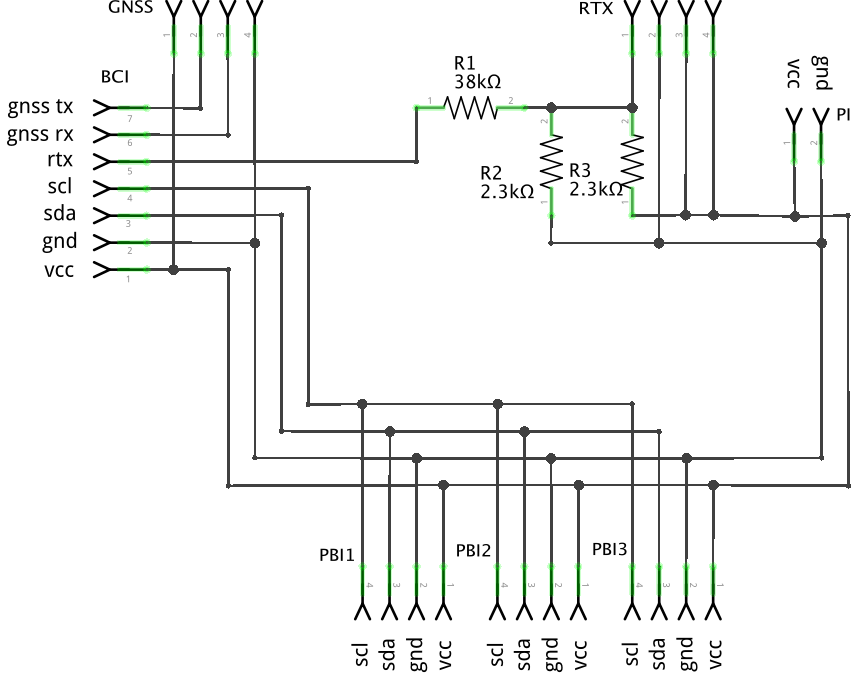
\includegraphics[width=0.4\textwidth]{ahabus-schema.png}
\centering
\caption{AHABus - Electronic Circuit}
\label{fig:ahabus-schema}
\end{figure}

Some preliminary printed circuit board layouts were designed for a next round
of testing. The schematics and the PCB layout are shown in figures
\ref{fig:ahabus-schema} and \ref{fig:ahabus-pcb}.

\begin{figure}[H]
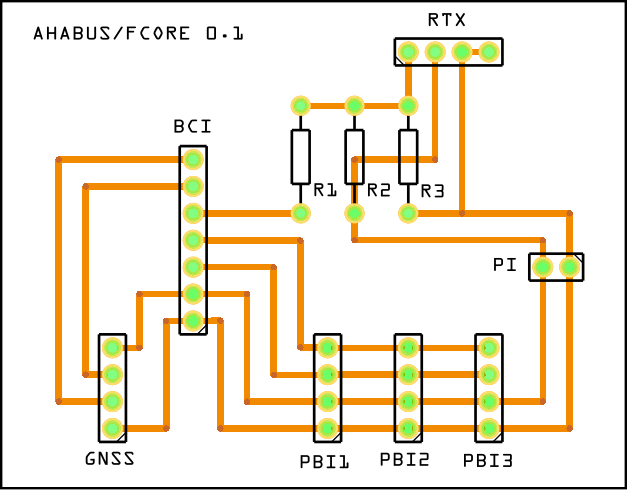
\includegraphics[width=0.4\textwidth]{ahabus-pcb.png}
\centering
\caption{AHABus - Printed Circuit Board Layout}
\label{fig:ahabus-pcb}
\end{figure}

\section{Ground Segment}
\label{sec:ground-segment}

\subsection{Extracting Raw Binary Stream}
\label{sec:binary-extraction}

The ground segment was based on Dl-Fldigi, an open-source binary radio decoder.
While Dl-Fldigi can decode RTTY signals, it was meant to decode RTTY text and
not binary data like the \acrshort{ahabus} packet radio protocol requires.
The data decoded by the software is not written to any file, but instead printed
in the main window, which means that byte which values are outside the range of
ASCII printable characters were invisible.

In order to allow a decoding tool to work on the full binary stream, a fork of
Dl-Fldigi was modified so that the binary stream could be extracted. When the
modified version starts, it creates a local network socket, to which any
byte decoded from RTTY streams are forwarded. This design was chosen because
most programming languages provide support for network communications, which
means that tools could easily be written to work with AHABus frame streams, such
as the packet parser discussed in the following section.

\subsection{Packet Parser}
\label{sec:packet-dispatcher}

For the purpose of debugging, a simple command-line based packet parser and
monitor was built upon the decoder discussed in section
\ref{sssec:rtx-decoder}. Because the platform was still at the prototype stage,
it was kept fairly simple. The location metadata contained in the packets is
displayed directly, as are system health packets. The data contained in packets
coming from payloads is written directly to one file for each payload. Listing
\ref{lst:fcore-parser-out} shows an example output from the packet parser.

\begin{lstlisting}[
    caption=Ground Segment - Example Packet Parser Output,
    label=lst:fcore-parser-out
]
[1490711516]: frame start detected
[1490711531]: decoded valid payload packet (0x14)
[1490711531]: 	>>>> FIX(56.462000deg, -2.970700deg, 5579m)
[1490711531]: rx stats: 7569 received, 7424/0 frame bytes (0 fixed)
[1490711545]: frame start detected
[1490711559]: decoded valid system packet
[1490711559]: 	>>>> FIX(56.462000deg, -2.970700deg, 5747m)
[1490711559]: 	>>>> FCORE//SYS_HEALTH :: G/U,P0A/U,P14/U
[1490711559]: rx stats: 7830 received, 7680/0 frame bytes (0 fixed)
[1490711569]: frame start detected
\end{lstlisting}

For testing purposes, the parser was also set to output statistics on the amount
of data received, fixed errors and number of frames decoded or lost.

\section{Evaluation}
\label{sec:testing}

Evaluation and testing of the project proved difficult because of the nature
of the prototype: embedded systems provide little, if any way to debug and
observe code behaviour. Instead, most of the testing had to focus on the data
received by the ground segment. Nonetheless, testing was conducted through
two main methods discussed in this section.

For all tests, the experimental setup was kept consistent: an ESP8266
development board was used as the \acrshort{obc}, while two Arduino Uno boards
were connected as payloads, generating fake instrument data. A \SI{5}{\volt}
power supply was connected to the power lines.

\subsection{Day in the life Testing}
\label{ssec:method-ditl}

The day-in-the-life test was meant to simulate a full \acrshort{hab} mission,
in order to evaluate both the overall viability of the platform, and test the
performance of the \acrshort{ahabus} platform's subsystems.

In order to come as close as possible to real-life conditions, the
\acrshort{gnss} receiver was replaced with an Arduino board programmed to
simulate the position updates of a receiver attached to a \acrlong{hab}
throughout ascent and descent.

Because the test was executed locally, the long-range aspect of the radio
communications could only be simulated by using a short antenna on the reception
side, and no antenna on the simulated platform.

\subsection{Resilience Testing}
\label{ssec:method-resilience}

The goal of the resilience tests was to test the performance of the packet radio
protocol, and specifically the \acrlong{fec}/Frame layer. To simulate a noisy
radio channel, a modified version of \acrshort{fcore} was built so that it
would randomly change the value of a byte before transmitting it. Knowing the
maximum theoretical correction limit of the \acrshort{fec} algorithm
($\frac{16}{256}$), three average error rates
($\frac{corrupted}{transmitted}$) were tested:

\begin{itemize}
    \item well under the limit ($\frac{8}{256}$);
    \item just under the limit ($\frac{14}{256}$);
    \item above the limit ($\frac{18}{256}$).
\end{itemize}

Each test involved having the prototype platform run for ten minutes in normal
conditions, an attempting to decode packets using ground segment software.
